\section{29.02.24 : }

\subsection{Grupa podstawowa $S^1$}

O okręgu możemy myśleć jako o podzbiorze $\R^2$
$$S^1=\{(x, y)\;:\;x^2+y^2=1\}$$
lub jako o podzbiorze $\C$:
$$S^1=\{z\;:\;|z|=1\}$$
Jest to oczywiście zbiór łukowo spójny, więc wybór punktu bazowego nie jest istotny. Dla wygody wybierzemy $x_0=(1, 0)$:
\begin{center}
  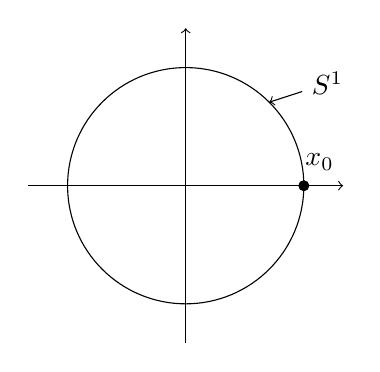
\begin{tikzpicture}
    \draw[->] (0, -2)--(0, 2);
    \draw[->] (-2, 0)--(2, 0);
    \draw (0,0) circle (1.5);
    \fill (1.5, 0) circle (2pt);
    \node at (1.7, 0.3) {$x_0$};
    \node (S) at (1.8, 1.3) {$S^1$};
    \draw[->] (S)--(45:1.5);
  \end{tikzpicture}
\end{center}
Rozważmy rodzinę pętli w $(S^1, x_0)$ indeksowaną przez $n\in\Z$:
$$w_n(s)=(\cos(2\pi ns),sin(2\pi ns))=e^{i2\pi ns},$$
gdzie $w_0\equiv x_0$ jest pętlą stałą.

\begin{theorem}[grupa podstawowa $S^1$]
  Odwzorowanie $\phi:(\Z, +)\to \pi_1(S^1, x_0)$ zadane przez $\phi(n)=[w_n]$ jest izomorfizmem.
\end{theorem}

Zanim jednak przejdziemy dalej, kilka uwag. Zacznijmy od tego, że 
$$\pi_1(S^{k-1})=\begin{cases}\Z&k=2\\ 0&k>2\end{cases}.$$
Z tego szybko możemy otrzymać
$$\pi_1(\R^k\setminus \{0\})=\pi_1(S^{k-1}\times \R)=\pi_1(S^{k-1})\times\pi_1(\R)=0\times 0,$$
czyli $\R^2$ nie jest homeomorficzne z $\R^n$ dla $n>2$.

Ponieważ $\phi$ jak wyżej jest izomorfizmem, to pętle $w_n$ są parami niehomotopijne. Co więcej, każda pętla w $S^1$ jest postaci $w_n$. Natomiast z działania na $\Z$ oraz homotopijności $\phi$ wiemy, że $w_nw_m=w_{n+m}$.

\begin{proof}
  Rozważmy pomocnicze ciągłe $p:\R\to S^1$ określone 
  $$p(t)=(\cos2\pi t, \sin 2\pi t)=e^{2\pi it}.$$
  Rozważmy też odwzorowanie 
  $$\overline{w_n}:[0,1]\to \R$$
\end{proof}
